
\documentclass[11pt,a4paper,computermodern]{article}


\usepackage[
%	includeheadfoot,
	width=172mm,
	top=18mm,
	bottom=18mm,
	bindingoffset=4mm
	]{geometry}



%%% Typeface packages
\usepackage[utf8]{inputenc}
\usepackage[T1]{fontenc}
\usepackage{fontawesome}

\usepackage{multirow}
\usepackage{tabularx}
\usepackage{booktabs}
\usepackage[flushleft]{threeparttable}

%%% Graphics packages
\usepackage{graphicx}



%%

\usepackage[
sorting=none,
backend=bibtex,
style=nature,
url=false,        
doi=false,         
isbn=false,
minbibnames=1,  
maxbibnames=10
]{biblatex} 

%%
%\newcommand{\code}[1]{\colorbox{light-gray}{\texttt{#1}}}
\newcommand{\code}{\texttt}

%%
\title{A Proposal for Stripe's Data Architecture}
\date{}


\begin{document}

\maketitle

\vspace{-10mm}

Stripe is a financial services company which provides payment processing solutions through APIs that web developers can use in their websites or mobile applications. The company processes billions of transactions annually, supporting millions of merchants worldwide.

The sensitive nature of the data managed by Stripe, along with the need of efficient


\section*{Data Pipeline}

Les données recueillies sont transférées depuis l'API de paiement utilisée par les sites marchands. On en distingue deux types:
\begin{itemize}
	\item A chaque transaction bancaire effectuée, un relevé est envoyé 
	\item Des données de télémétrie sont transférées
\end{itemize}


\section*{Online Transaction Processing Model}

Our proposed OLTP database architecture is presented in figure~\ref{fig:OLTP}. The core of the database is a registry of all financial transactions occurring within Stripe scope. Additional tables contain information about merchants and customers. Fraud indicators are stored in a dedicated table in a one-to-one correspondence with the main transactions table. The rationale behind this choice is that fraud indicators do not originate from the same source as transactions, and are not produced at the same time.


\begin{figure}
	\centering
	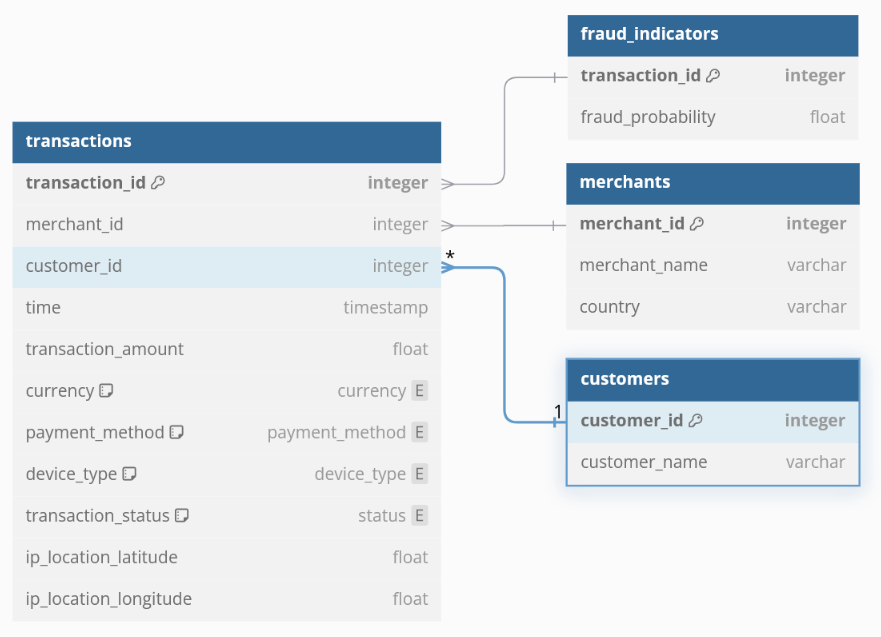
\includegraphics[scale=0.7]{./figures/OLTP}
	\caption{Proposed OLTP database structure.}
	\label{fig:OLTP}
\end{figure}


\begin{table}[ht]
	\centering
	\begin{threeparttable}
		\caption{Data dictionary for the \code{transactions} OLTP schema.}
		\label{table:OLTP}
		\begin{tabularx}{0.99\textwidth}{c c >{\centering\arraybackslash}X >{\centering\arraybackslash}X}
			\toprule
			Field Name & Type & Description & Example  \\
			\midrule
			\multicolumn{4}{c}{\code{transactions} table}\\
			\code{transaction\_id} & \code{bigint} & Unique transaction id & \code{123456789} \\
			\code{merchant\_id} & \code{bigint} & Merchant id & \code{12345} \\
			\code{customer\_id} & \code{bigint} & Customer id & \code{234567} \\
			\code{time} & \code{datetime} & UTC transaction timestamp & \code{2023-11-18 17:43:02.4} \\
			\code{amount} & \code{decimal(10,2)} & Transaction amount (in currency unit) & \code{43.15} \\
			\code{currency\_code} & \code{char(3)} & Currency code (ISO 4217) & \code{'GBP'} \\
			\code{payment\_method} & \code{varchar(16)} & Payment method & \code{'credit\_card'} \\
			\code{device\_type} & \code{varchar(16)} & Device used for payment & \code{'mobile'} \\
			\code{status} & \code{varchar(16)} & Transaction status & \code{'sucess'} \\
			\code{ip\_latitude} & \code{float} & IP-based geolocation latitude & \code{49.6833300} \\
			\code{ip\_longitude} & \code{float} & IP-based geolocation longitude & \code{10.5333300} \\
			\midrule
			\multicolumn{4}{c}{\code{merchants} table}\\
			\code{merchant\_id} & \code{bigint} & Unique merchant id & \code{12345} \\
			\code{name} & \code{varchar} & Merchant name & \code{'Amazon UK'} \\
			\code{iban} & \code{varchar} & Merchant IBAN & \code{'GB82WEST12345678765432'} \\
			\code{country\_code} & \code{char(2)} & Merchant registration country code & \code{'GB'} \\
			\midrule
			\multicolumn{4}{c}{\code{customers} table}\\
			\code{customer\_id} & \code{bigint} & Unique customer id & \code{234567} \\
			\code{name} & \code{varchar} & Customer name & \code{'John Doe'} \\
			\code{iban} & \code{varchar} & Customer IBAN & \code{'GB82WEST12345678765432'} \\
			\code{country\_code} & \code{char(2)} & Customer country code  & \code{'GB'} \\
			\midrule
			\multicolumn{4}{c}{\code{fraud\_indicators} table}\\
			\code{transaction\_id} & \code{bigint} & Transaction id & \code{123456789} \\
			\code{fraud\_probability} & \code{float} & Fraud probability & \code{0.12} \\
			\bottomrule
		\end{tabularx}
	\end{threeparttable}
\end{table}


\section*{Online Analytical Processing Model}

Pour l'analyse et la préparation de features pour la détection de fraude, on utilisera une base 


\begin{figure}
	\centering
	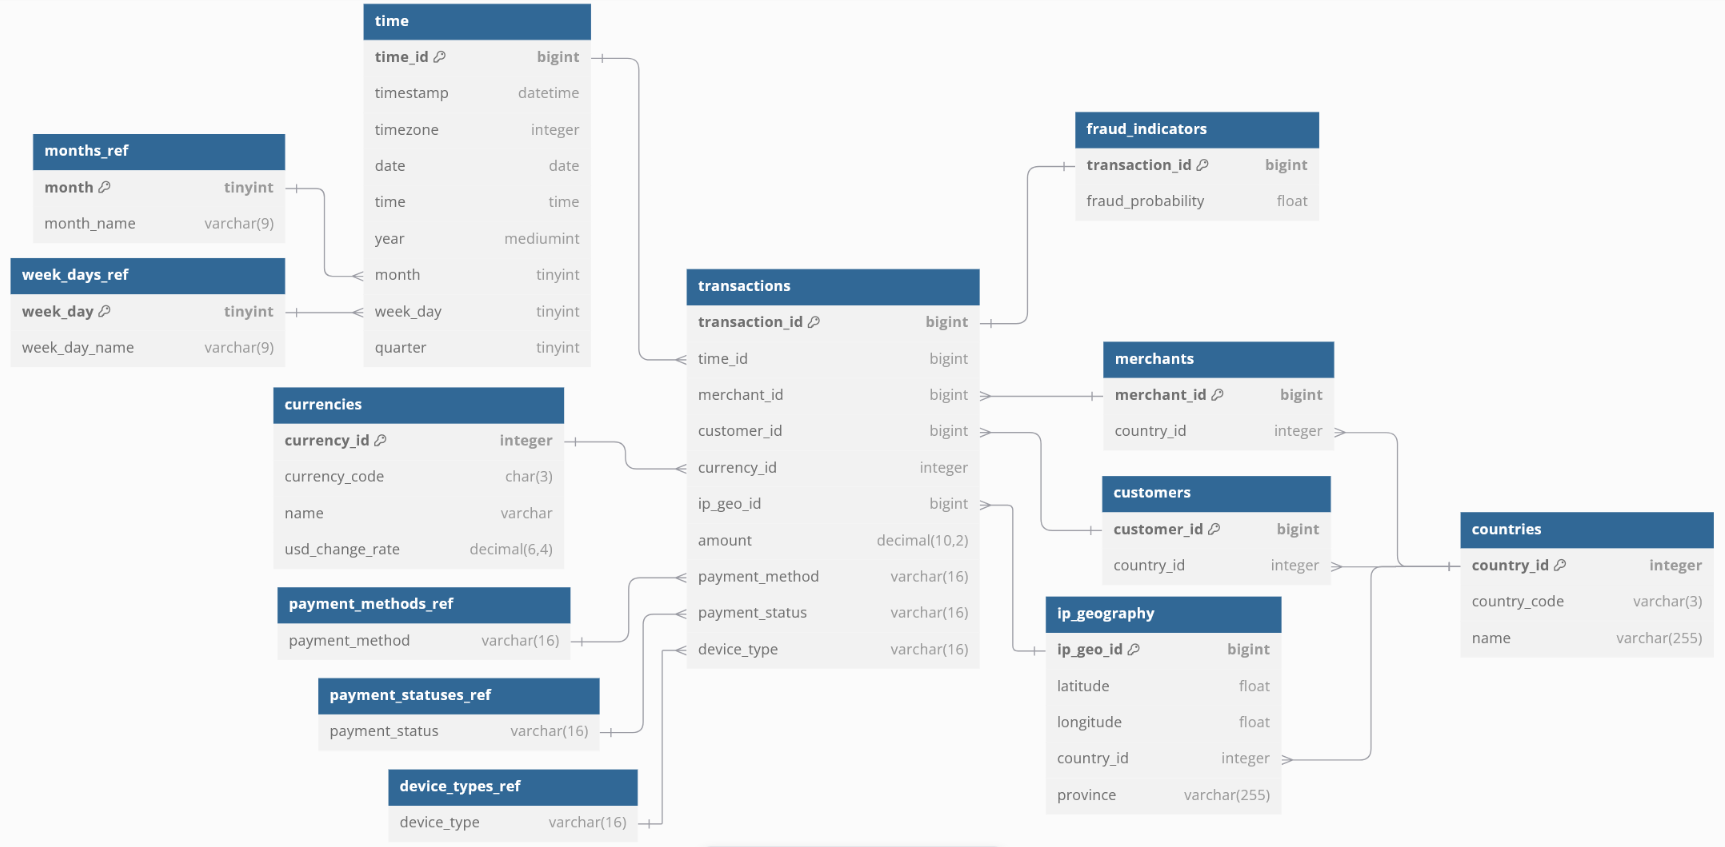
\includegraphics[scale=0.46]{./figures/OLAP}
	\caption{Proposed OLAP database structure.}
	\label{fig:OLAP}
\end{figure}


\begin{table}[ht]
	\centering
	\begin{threeparttable}
		\caption{Data dictionary for the main tables in \code{transactions} OLAP schema.}
		\label{table:OLAP_main}
		\begin{tabularx}{0.99\textwidth}{c c >{\centering\arraybackslash}X >{\centering\arraybackslash}X}
			\toprule
			Field Name & Type & Description & Example  \\
			\midrule
			\multicolumn{4}{c}{\code{transactions} table}\\
			\code{transaction\_id} & \code{bigint} & Unique transaction id & \code{123456789} \\
			\code{time\_id} & \code{bigint} & Transaction time id & \code{123456789} \\
			\code{merchant\_id} & \code{bigint} & Merchant id & \code{12345} \\
			\code{customer\_id} & \code{bigint} & Customer id & \code{234567} \\
			\code{currency\_code} & \code{char(3)} & Currency code (ISO 4217) & \code{'GBP'} \\
			\code{ip\_geo\_id} & \code{bigint} & IP geolocalization id & \code{1234567} \\
			\code{payment\_method\_id} & \code{integer} & Payment method id & \code{1} \\
			\code{payment\_status\_id} & \code{integer} & Payment status id & \code{2} \\
			\code{device\_type\_id} & \code{integer} & Device id & \code{3} \\
			\code{amount} & \code{decimal(10,2)} & Transaction amount (in currency unit) & \code{43.15} \\
			
			\midrule
			\multicolumn{4}{c}{\code{time} table}\\
			\code{time\_id} & \code{bigint} & Unique transaction time id & \code{123456789} \\
			\code{timestamp} & \code{datetime} & UTC transaction timestamp & \code{2023-11-18 17:43:02.4} \\
			\code{timezone} & \code{integer} & Timezone offset in minutes & \code{-120} for UTC-02:00 \\
			\code{date} & \code{date} & Transaction date & \code{2023-11-18} \\
			\code{time} & \code{time} & UTC transaction time & \code{17:43:02.4} \\
			\code{year} & \code{mediumint} & Transaction year & \code{2023} \\
			\code{month} & \code{tinyint} & Transaction month & \code{11} \\
			\code{week\_day} & \code{tinyint} & Transaction week day (\code{0} is sunday) & \code{6} (saturday) \\
			\code{quarter} & \code{tinyint} & Transaction quarter & \code{4} \\
			
			\midrule
			\multicolumn{4}{c}{\code{merchants} table}\\
			\code{merchant\_id} & \code{bigint} & Unique merchant id & \code{12345} \\
			\code{country\_code} & \code{char(2)} & Merchant registration country code & \code{'GB'} \\
			
			\midrule
			\multicolumn{4}{c}{\code{customers} table}\\
			\code{customer\_id} & \code{bigint} & Unique customer id & \code{234567} \\
			\code{country\_code} & \code{char(2)} & Customer country code & \code{'GB'} \\
			
			\midrule
			\multicolumn{4}{c}{\code{fraud\_indicators} table}\\
			\code{transaction\_id} & \code{bigint} & Transaction id & \code{123456789} \\
			\code{fraud\_probability} & \code{float} & Fraud probability & \code{0.12} \\
			
			\midrule
			\multicolumn{4}{c}{\code{ip\_geography} table}\\
			\code{ip\_geo\_id} & \code{bigint} & Geolocation id & \code{123456789} \\
			\code{latitude} & \code{float} & IP-based geolocation latitude & \code{49.6833300} \\
			\code{longitude} & \code{float} & IP-based geolocation longitude & \code{10.5333300} \\
			\code{country\_code} & \code{char(2)} & country code (ISO 3166-1 alpha-2) & \code{'DE'} \\
			\code{province} & \code{varchar(255)} & Province name & \code{'Darmstadt'} \\
			
			\bottomrule
		\end{tabularx}
	\end{threeparttable}
\end{table}


\begin{table}[ht]
	\centering
	\begin{threeparttable}
		\caption{Data dictionary for the reference tables in \code{transactions} OLAP schema.}
		\label{table:OLAP_ref}
		\begin{tabularx}{0.99\textwidth}{c c >{\centering\arraybackslash}X >{\centering\arraybackslash}X}
			\toprule
			Field Name & Type & Description & Example  \\
			\midrule
			\multicolumn{4}{c}{\code{currencies} table}\\
			\code{currency\_code} & \code{char(3)} & Currency code (ISO 4217) & \code{'GBP'} \\
			\code{currency\_name} & \code{varchar(255)} & Currency name & \code{'Pound sterling'} \\
			\code{usd\_change\_rate} & \code{decimal(6,4)} & currency/USD change rate & \code{1.2479} \\
			
			\midrule
			\multicolumn{4}{c}{\code{countries} table}\\
			\code{country\_code} & \code{char(3)} & Country code (ISO 3166-1 alpha-2) & \code{'GB'} \\
			\code{country\_name} & \code{varchar(255)} & Country name & \code{'United Kingdom'} \\
			
			\midrule
			\multicolumn{4}{c}{\code{payment\_methods} table}\\
			\code{payment\_method\_id} & \code{integer} & Unique payment method id & \code{1} \\
			\code{payment\_method} & \code{varchar(16)} & Payment method & \code{'credit\_card'} \\
			
			\midrule
			\multicolumn{4}{c}{\code{payment\_statuses} table}\\
			\code{payment\_status\_id} & \code{integer} & Unique payment status id & \code{1} \\
			\code{payment\_status} & \code{varchar(16)} & Payment status & \code{'sucessful'} \\
			
			\midrule
			\multicolumn{4}{c}{\code{device\_types} table}\\
			\code{device\_type\_id} & \code{integer} & Unique device type id & \code{1} \\
			\code{device\_type} & \code{varchar(16)} & Device type & \code{'mobile'} \\
			
			\midrule
			\multicolumn{4}{c}{\code{months} table}\\
			\code{month} & \code{tinyint} & Month number & \code{11} \\
			\code{payment\_status} & \code{varchar(9)} & Month name & \code{'november'} \\
			
			\midrule
			\multicolumn{4}{c}{\code{week\_days} table}\\
			\code{week\_day} & \code{tinyint} & Week day number & \code{6} \\
			\code{week\_day\_name} & \code{varchar(9)} & Day name & \code{'saturday'} \\
			
			\bottomrule
		\end{tabularx}
	\end{threeparttable}
\end{table}


\section*{NoSQL Model}

L'entreprise doit aussi gérer des données semi-structurées telles que les fichiers de log, les reçus de transactions ou encore la télémétrie effectuée sur la plateforme de paiement. Les contraintes pour chaque catégorie de données sont diverses et on adoptera une solution adaptée à chacune.

\begin{itemize}
	\item Les informations de session ayant principalement des contraintes de disponibilité associée à des requêtes simples, on s'orientera vers une database de type key-value.
	\item Les fichiers de log sont structurés comme une succession d'évènements. Ceux-ci doivent être stockés de façon à pouvoir alimenter en temps réel des algorithmes de détection d'anomalies, afin d'assurer une réponse rapide en cas d'incident. Il est aussi nécessaire qu'ils soient lisibles par un humain pour une analyse approfondie. On s'orientera donc naturellement vers une document-based NoSQL database pour ce cas d'usage.
	\item Les fichiers non sensibles peuvent être stockés dans un espace approprié (Amazon S3) et indexés par une document-based database qui contiendra aussi les métadonnées.
	\item La télémétrie dans une column database
	\item Les features pour le machine learning peuvent être stockés dans une graph database.
\end{itemize}


\section*{Security and Compliance}

The company stores sensitive user data such as banking information. Il est important de sécuriser ces donnees pour deux raisons. D'une part, pour etre en accord avec la legislation locale (eg GDPR). D'autre part, la fuite de ces données impacterait la confiance accordée à l'entreprise par ses clients, avec en conséquence une baisse potentielle des revenus. Afin de limiter la surface d'attaque possible, les données sensibles sont confinées dans la base OLTP, et chiffrées à l'interieur de celle-ci.

Il est nécessaire de reporter en partie de ces données dans la base OLAP, notamment pour l'étude des délits financiers (fraude, blanchiment, etc). Afin de limiter les risques, la base OLAP ne continent que des éléments anonymisés de ces données, telles que la localisation ou le nom de la banque. Afin de maintenir la performance du système, ces données ne sont pas chiffrées et on se limitera à en sécuriser l'accès et le transfert (définition de roles pour limiter l'accès, etc). De la même façon, aucune donnée sensible n'est stockée directement dans la base NoSQL.

On distinguera les fichiers selon leurs contraintes en termes de sécurité. Les fichiers sensibles tels que les reçus bancaires seront stockés dans un datalake dédié avec un accès restreint. Ils seront indexés exclusivement dans la base OLTP (non indiqué sur le schéma). Les autres fichiers seront de la même façon enregistrés dans un datalake et indexés dans la base NoSQL dédiée.

Des backups chiffrés sont mis à jour à intervalles réguliers afin d'assurer le rétablissement du service en cas d'incident majeur.

Enfin, un système de log est mis en place afin d'enregistrer toutes les connexions aux serveurs, les accès aux données, les requêtes effectuées, etc. Un service additionnel peut être mis en place afin de détecter les anomalies en temps réel.


\section*{Machine learning integration}



\vspace{.0cm}
\section*{References}



\end{document}